\chapter{Usability}
\section{Usability}
Usability says something about how easy it is to use, learn and understand a human-made system. Examples of systems can be a machines, software applications, websites, tools, or anything else that involves human interaction with an object. Usability is a often used in association with technology development, in terms of making digital systems understandable and intuitive for the users through user-friendly interfaces. Usability has played a huge part in the evolvement of bringing digital systems into people’s homes and everyday life. The first computers and digital systems that were developed consisted of complex and not understandable applications that only professionals with special knowledge could use. There was little focus on simple and accessible systems, and complex interfaces were actually appreciated and gave the system credibility. First, when computers and digital systems were developed with the intention of being used by the normal user, developers had to think about usability. The developers had to put the user in the center of the computer system, and not only focus on functionality and system features \cite{mmi}.

Usability is a wide and quite abstract term, and it is not easy to understand, to measure, or to practise right. There is no definitive solution on how to make a good and user friendly system, and it is challenging and time consuming to find the users needs. For a system design to experience success interaction designers has to pay attention to various aspects of the user. The best way to do this is to involve users in the process of developing the system, from requirement definition and the design phase, to prototype and system test, all to the end of the system's lifecycle \cite{mmi}. When creating something completely new, it is all about understanding what the users want and need, but often the users themselves do not know what they want. It will not be possible to walk up to a potential customer and ask what he or she wants and needs. This does not mean that a developer should be creative, come up with a great idea and bring it into life without ever talking to the user group. The development of a new system should be done as a cyclic process, where development and user involvement goes hand in hand \cite{mmi}.  
\begin{figure} [ht!]
\centering
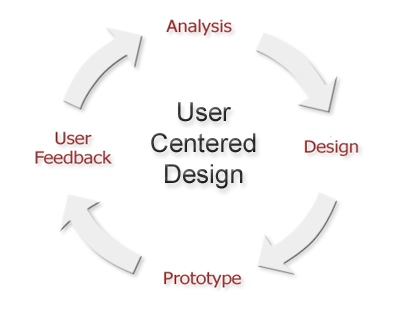
\includegraphics[scale=0.8]{userdesign.jpg}
\caption{User Centered Design \cite{userdesign}}
\label{userdesign}
\end{figure}

Making good, intuitive, easy to understand systems is essential for a system to be successful, accepted and used. "Make it or break it" is a slogan that connects well with success and acceptance. A system can possess the best functionality there is, but if the users do not understand how to use it, the system will fail. An example of this is Apple's huge breakthrough when they launched their iPhone in 2007 \cite{iphone2007}. One might associate the invention of the touch phone with Apple's iPhone, but the truth is that touch phones was invented long before the iPhone. The first touch screen was published as early as in 1968, where it was used for air traffic control. In the early 1990s IBM released their Simon, which was the first smart phone with touch screen technology \cite{touchphone}. Apple was also eager participants in the development of touch screen devices. Already in 1983 Apple had a prototype of a touch screen phone \cite{applefirst1983}, and in 1993 they released the world's first Personal Digital Assistant (PDA), called Newton \cite{touchphone}. Apple’s success with their iPhone is based on focus on user’s needs throughout the development process, which has resulted in good, intuitive and user-friendly design and interfaces. "KISS" and "Less is more" is other terms related to usability. "KISS" is an acronym that stands for "Keep it simple, stupid". This term was used in the US navy in the 1960's, and it was a principle stating that simple systems work best than complex ones. The KISS principle has been adopted into the subject of design and usability. Simplicity should be the main focus in design, and every element that leads to unnecessary complexity should be avoided [KILDE - wiki foreløpig]. Ludwig Mies van der Rohe was a German architect that used the term "Less is more" to describe his extreme simplistic and minimalistic design style, and his use of that term became a guiding principle in modern design. "Less is more" has also been widely used as a slogan in association with usability. \cite{rohe}. Minimalistic design can be described as "design at its most basic, stripped of superfluous elements, colors, shapes and textures." With minimalistic design, the most important elements are brought into focus. In this way the user will not be distracted from, or miss out on, the content that is important \cite{lessismore}. Also big companies, like Microsoft, focus on simplicity in their design. Microsoft has launched an article called "The Importance of Simplicity" in their developer network, about how to design user-friendly systems while still keeping good functionality. Microsoft present a topic called "Simple Can Be Powerful". This means that simplistic design not necessarily implies lack of functionality. Simplistic design will provide ease of use for first timers. The idea is to present a design that is intuitive, understandable and easy to learn, but that has the opportunity to build up knowledge about the functionality needed. A possible solution could be to include customisation so the users can set up their own workspace \cite{msdnsimple}.             

We have experienced a great shift in technology from the first computer was invented and until today. Technology has been more mobile due to laptops, smart phones and other portable devices, and it is also used more often because of instant messaging, e-business and social networks \cite{mmi}. Users are no longer just "computer professionals", but normal people in all age groups, with different skills and interests, that are both experienced and inexperienced with technology. This has been possible because of designers and researchers with focus on human needs. The term human-computer interaction was created, which is about including psychology in developing human-centric design. This is not an easy task, and it includes people from a many different sciences. Ben Shneiderman list “psychologist, instructional and graphic designers, technical writers, experts in human factors or ergonomics, information architects, and adventuresome anthropoplogists and sociologist” as some of the people to be included in the process of saying something about usability and human-computer interaction \cite{mmi}.    

The work for an interactive system designer is as mentioned to combine the sense of what attracts users with system functionality. To help interface designers make successful systems, a theory called the four pillars of design has been developed. This theory does not guaranteed brilliant systems, but it could be helpful along the way in making good, successful systems. The four pillars of design consist of “user-interface requirements”, “guidelines, documents and processes”, “user-interface software tools” and “expert reviews and usability testing” \cite{mmi}.    

\emph{User-interface requirements (Ethnographic observations)}\\
A major key to success when developing a system is connected to specifying the user requirements, and how well these requirements are defined and understood.  The way to specify requirements differs from organisation to organisation, but what the final results should always include the same; Who should use the system, where should it be used and what should it be used for. In addition to this, functional requirements (system requirements like hardware,  software etc.) and non-functional requirements (requirements saying something about the user interface, like functionality, input devices, etc.) should be specified and decided \cite{mmi}.

\emph{Guidelines documents and process (Theories and models)}\\
It is important for the interactive system designer to generate a document that obtains a set of guidelines which specifies how the design should be. Companies like e.g. Apple uses guidelines documents to specify design principles developers should follow. This is to create consistency in design across systems and products. Design may differ as different systems has different needs, but there are still some elements that should be considered in the guidelines document. The documents should contain guidelines for:

\begin{itemize}
\renewcommand{\labelitemi}{$\bullet$}
\item Words, icons, and graphics.
\item Screen-layout issues.
\item Input and output devices.
\item Action sequences.
\item Training.
\end{itemize}

The procedure of creating these guidelines should be done by including different parts of an organisation. It should be a social process, this to gain visibility. It is important that the guidelines are flexible, so that they can adapt to changes in needs and experiences \cite{mmi}. 

\emph{User-interface software tools (Algorithms and prototypes)}\\
In the early stages of development, it is difficult for users to picture what the final result will look like. This may lead to situations where the system design is finished and the users are left with the feeling of not being satisfied. This would be a problem, because of the high cost associated to make changes in implemented systems. One way to address this problem is to let the users get a realistic impression of the final result early in the development process. This could be done by presenting different types of prototypes. These prototypes could be simple sketches on paper, a display proposal or a presentation with use of PowerPoint. 
When deciding on which development environment to use, there is a number of good products to choose from. Most of them are easy to use, and offers good features. The important part is for the developers to choose the development environment that is most suitable for the product they are going to make, due to performance, cost, and how easy it is to use and learn \cite{mmi}.
	
\emph{Expert reviews and usability testing (Controlled experiments)}\\
To be able to launch a successful system, it is important with testing along the way in the development process. System testing could involve both experts and the intended users \cite{mmi}. 

With the importance of user friendly technology systems, as well as user involvement, in mind, we will move on to the next chapter, where we will describe the methodology used in this thesis. 